\chapter{Desenvolvimento}
\label{chapter:desenvolvimento}
% https://www.freecodecamp.org/news/how-to-start-an-open-source-project-in-new-years-945bad8800d7/
% https://www.linuxfoundation.org/resources/open-source-guides/starting-open-source-project/#7
% https://opensource.guide/starting-a-project/#your-pre-launch-checklist
% https://americanexpress.io/on-the-importance-of-commit-messages/
% https://dev.to/maniflames/how-conventional-commits-improved-my-git-skills-1jfk
% https://www.conventionalcommits.org/en/v1.0.0/
% https://medium.com/@andrewhowdencom/anatomy-of-a-good-commit-message-acd9c4490437


% \section{Importância do uso de convenções}
% Não sei como escrever essa parte aqui

\section{O uso do Git}
\label{git_usage_section}

O Git é uma ferramenta bastante poderosa e de fácil uso em sua forma básica, porém seu uso pode se tornar bastante complexo ao se usar funcionalidades mais avançadas. O objetivo desta seção é introduzir elementos e conceitos presentes no restante do trabalho, para garantir um melhor entendimento dos conceitos.

Seja individualmente ou de forma colaborativa, o uso da ferramenta Git gira em torno de três funções fundamentais: \textit{commits}, \textit{branches} e interações com outros repositórios. Cada uma dessas permite, respectivamente, o versionamento, o trabalho em paralelo e o controle de versionamento distribuído.

% o que é um commit
\textit{Commit} é o nome dado para cada versão que o usuário cria com a ferramenta. Um \textit{commit} é formado por: uma hash de identificação criada pelo Git, a identificação do autor, data de criação, uma mensagem associada, a \textit{hash} do \textit{commit} pai e da \textit{branch} a qual o mesmo pertence, além das modificações realizadas. 

Essas versões podem ser acessadas à qualquer momento pelo desenvolvedor, por meio da hash identificadora de cada \textit{commit}. O Git é capaz de listar todas as versões que se possui até aquele momento a partir do commando \textbf{git log} como pode ser visto na Figura \ref{fig:commit_example}.

Nessa exibição, as alterações realizadas - chamadas dentro da ferramenta de \textit{diff} - são ocultadas para o usuário, assim sendo, se torna perceptível a importância da mensagem presente em um \textit{commit}. Mais adiante, boas práticas e conceitos relacionados ao \textit{commit} serão melhor abordados na Seção \ref{section:commit}. % \cite{mastering_git}

\begin{figure}[h]
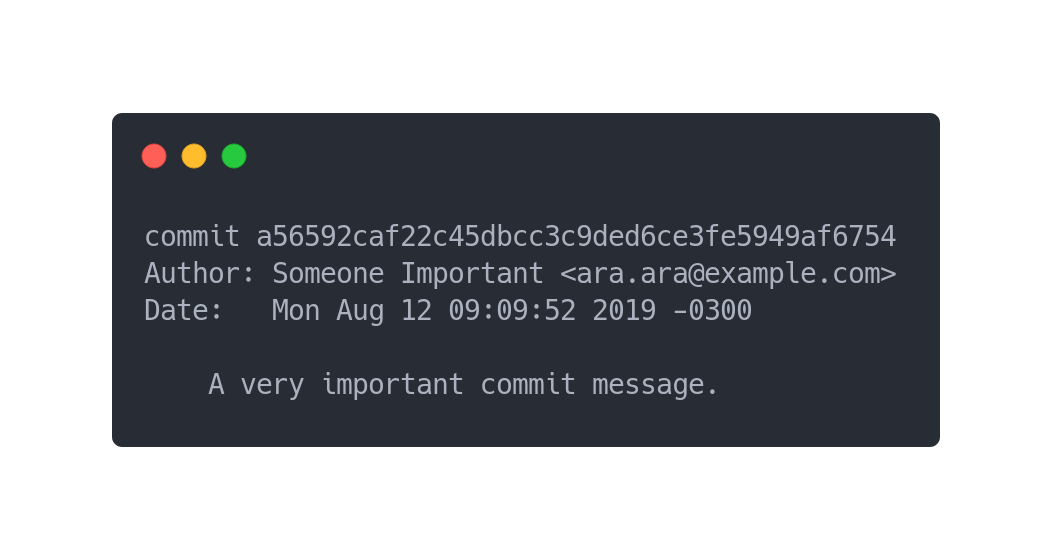
\includegraphics[width=12cm]{figuras/carbon.png}
\centering
\label{fig:commit_example}
\caption{Exemplo de um commit como visto em um \textbf{git log}.}
\end{figure}

% o que são branches
Um outro conceito fundamental do Git são as \textit{branches}. Uma \textit{branch} funciona como uma lista ligada de \textit{commits}, já que cada um possui a referência do seu anterior. Por padrão, o Git proporciona ao usuário uma \textit{branch} padrão, chamada \textit{master}. Essa branch é criada junto ao primeiro \textit{commit} de um repositório. O uso de \textit{branches} permite o desenvolvimento paralelo de diversas atividades dentro de um repositório de trabalho.

Relacionado as \textit{branches}, está a árvore de \textit{commits}. Ela é uma forma de visualizar as \textit{branches} e seus respectivos \textit{commits}. Uma representação de uma árvore de \textit{commits} - ou \textit{commit tree} - pode ser vista na Figura \ref{fig:git_tree}.  A utilização de \textit{branches} é um dos pilares principais que suportam a capacidade do Git de permitir trabalho simultâneo e colaborativo, visto que cada colaborador pode realizar alterações em sua \textit{branch} sem interferir com o trabalho de outro.

% http://jsfiddle.net/fracz/q76vj8ow/

\textit{Branches} também são extremamente importantes para uma boa organização do repositório, geralmente possuindo em repositórios de software sua própria política a ser seguida pelos contribuidores.

\begin{figure}[b]
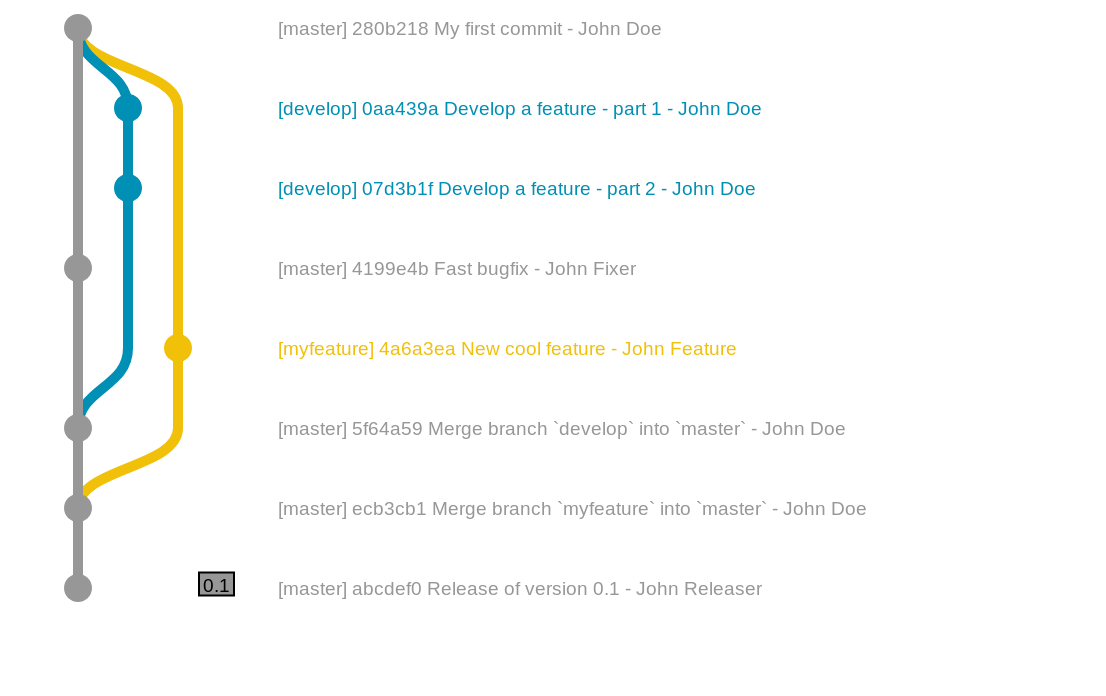
\includegraphics[width=12cm]{figuras/gittree.png}
\centering
\label{fig:git_tree}
\caption{Exemplo de uma \textit{git tree} com 3 \textit{branches}. Cada ponto representa um \textit{commit} e cada cor representa uma \textit{branch} diferente. Fonte: http://jsfiddle.net/fracz/q76vj8ow/}
\end{figure}


% como se dá a interação com outros repositórios
Por se tratar de um sistema de versionamento distribuído, o Git possui ferramentas de gerenciamento de repositórios, permitindo que o usuário gerencie as mudanças realizadas no seu repositório local e as submeta para o repositório em um servidor e vice-versa. O Git realiza tais ações por meio da mesclagem de \textit{branches}. Essa mesclagem pode ocorrer entre \textit{branches} presentes no repositório local e entre \textit{branches} localizadas no repositório local e na nuvem.

% O Git é uma ferramenta bastante poderosa e de fácil uso em sua forma básica, porém seu uso pode se tornar bastante complexo ao se usar funcionalidades mais avançadas. O objetivo desta seção é introduzir elementos e conceitos presentes no restante do trabalho, para garantir um melhor entendimento dos conceitos.

% 
% 
% 
% 
% 
% 
% 
\newpage
\section{O \textit{commit}}
\label{section:commit}

\subsection{O uso de \textit{commits} como parte de documentação de software}
% documentação de software
É algo já estabelecido na área de engenharia e desenvolvimento de software a importância da documentação. Seja em forma de documentos, tutoriais, testes e diagramas ou seja na forma de artefatos menos formais, como \textit{issues} e discussões a cerca de código \cite{importance_of_software_documentation}.

Segundo Sommerville, a documentação de um produto de software faz parte do que é denominado software \cite{sommerville_o_que_eh_software}, portanto artefatos presentes no processo de desenvolvimento de software com o intuito de informar ou ajudar desenvolvedores ou colaboradores externos fazem parte da documentação do software por consequência.

% o que sao commits no git
Durante o processo de desenvolvimento de software, especialmente considerando a cultura de colaboração presente atualmente, desenvolvedores somos constantemente incentivados a versionar o código que trabalhamos.
A importância de tal prática é deveras considerável, visto que um bom gerenciamento de versões permite um controle maior nas alterações submetidas.
% Seja para facilitar a integração com as alterações de um outro colaborador, ou para sinalizar a inserção de uma nova funcionalidade, a importância de se versionar não é algo questionável.

Como dito préviamente, no cenário atual de desenvolvimento de software a principal ferramenta de versionamento utilizada é o Git. O sistema de versionamento do Git ocorre a partir de \textit{commits}.

% como commits se encaixam como documentação


\subsection{Principais boas práticas de \textit{commit}}

% importancia de bons commits

% o que é visto como boas práticas de commit pela comunidade

\subsection{Principais convenções de \textit{commit}}
\subsubsection{Convenção angular}

% referencias

% principais pontos da convenção

% exemplos de uso

% the good and the bad

\subsubsection{Convenção karma}

% referencias

% principais pontos da convenção

% exemplos de uso

% the good and the bad

\subsubsection{Convenção changelog}

% referencias

% principais pontos da convenção

% exemplos de uso

% the good and the bad

\subsubsection{Convenção symphony cmf}

% referencias

% principais pontos da convenção

% exemplos de uso

% the good and the bad


\subsection{Ferramentas de auxílio à escrita de \textit{commit} seguindo convenções}
\subsubsection{Commitzen}
\subsubsection{Commit Helper} % coloco aqui mesmo?




\newpage
\section{Convenções de repositórios de software}

\subsection{O \textit{git flow}}

\subsection{O \textit{semantic versioning}}

\subsection{Documentação padrão}



\newpage
\section{Proposta de trabalho}